\documentclass[../uilmath.tex]{subfiles}
\graphicspath{{\subfix{../figures/}}}
\begin{document}
\chapter{Geometry}
\section*{Problems}
\begin{enumerate}[label=\bfseries\arabic*.]
    \item %% Problem 1
    The sides of a triangle are 9 in, 12 in, and 15 in. The triangle is a(n) \blank triangle:

    \item %% Problem 2
    An isosceles trapezoid has a top base of 8 cm, a bottom base of 14 cm, and a slanted side length of 5 cm. Find the area of the isosceles trapezoid.

    \item %% Problem 3
    Rene drew $\triangle ABC$ using the coordinates $(1,2), (2,-2)$ and $(5,1)$. Find the area of Rene's triangle.

    \item %% Problem 4
    Georg Alexander picks the special figure and places it on a five-peg-by-five-peg geoboard. Find the area enclosed by the figure.
    \begin{center}
        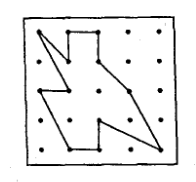
\includegraphics[width=0.3\textwidth]{2006SAC16.PNG}
    \end{center}

    \item %% Problem 5
    $\triangle DEF$ is an obtuse isosceles triangle such that m$\angle DEF$ is 104$\degree$ and EF is 14 cm. Find the area of $\triangle{DEF}$ to the nearest integer.

    \item %% Problem 6
    Point $P(3,3)$ is rotated 270$\degree$ counterclockwise about the origin to point $Q$. Point $Q$ is reflected across the $y$-axis to point $R$. Find the coordinates of point $R$.

    \item %% Problem 7
    Two chords, $AC$ and $BD$ intersect in the interior of a circle at point $X$ such that $m\arc{BC}=20\degree$ and $m\arc{AD}=120\degree$. If points $B$ and $C$ are not on $\arc{AD}$ then $m\angle AXD$ is:

    \item %% Problem 8
    The adjacent dots on the grid are 1 cm apart when measured vertically and horizontally. Find the area of the shaded figure shown.
    \begin{center}
        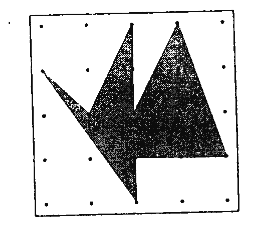
\includegraphics[width=0.3\textwidth]{2008SAC9.PNG}
    \end{center}

    \item %% Problem 9
    One of the base angles of an acute isosceles triangle has a measure of 50$\degree$ and the length of its base is 6 cm. Find the perimeter of the acute isosceles triangle. (nearest tenth)

    \item %% Problem 10
    The square below is divided into 5 congruent rectangles. The perimeter of each of the congruent rectangles is 30 units. What is the perimeter of the square?
    \begin{center}
        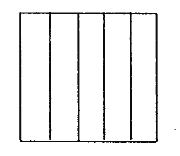
\includegraphics[width=0.3\textwidth]{2008SAC23.PNG}
    \end{center}

    \item %% Problem 11
    Simplify: $\frac{n!+(n-1)!}{(n-2)!}$

    \item %% Problem 12 
    Let $AB$ be the diameter of the circle with center $C$ with $CG\perp AB, DE\perp AB$, and $EF\perp DC$. 
    If $AE=9$ and $BE=4$ then $DE=$?
    \begin{center}
        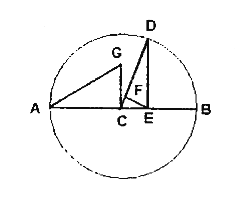
\includegraphics[width=0.3\textwidth]{2008SAC27.PNG}
    \end{center}

    \item %% Problem 13
    Given: $\triangle ABC \sim \triangle DEF, AB = 15, AC = 12, m\angle A = 62\degree, DE = 10$. $EF=\blank$. (nearest tenth)

    \item %% Problem 14
    Points $A$ and $B$ line on a circle with center $O$. The area of the circle is 531 and $AB=24$. Find the distance from $O$ to chord $\overline{AB}$. (nearest tenth)

    \item %% Problem 15
    Consider a circle circumscribed about a regular pentagon. If the area of the circle is 452.4, then the area of the pentagon is $\blank$. (nearest whole number)


    Use the sketch below for problems 16 and 17. The information given in problem 16 does not carry over to problem 17.
    \begin{center}
        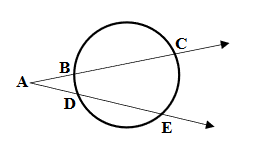
\includegraphics[width=0.3\textwidth]{2021SAC18.PNG}
    \end{center}
    \item %% Problem 16
    If $AB=6, BC=15$, and $AD=8$, then $DE=\blank$. (nearest hundredth)

    \item %% Problem 17
    If $mBD = 28\degree$ and $mCE = 86\degree$, then $m\angle CAE=\blank$.$\degree$

    \item %% Problem 18
    The base of a pyramid is a square with each side equal to three-fifths of the height of the pyramid. If the volume 
    of the pyramid is 700, what is the total area of the pyramid? (nearest whole number)

    \item %% Problem 19
    Angles $A$ and $B$ are complementary angles while angles $A$ and $C$ are supplementary angles. If 
    $m\angle A = 6x+1$ and $m\angle B = 9x-1$, then $m\angle C = \blank\degree$.

    \item %% Problem 20
    Quadrilateral $ABCD$ shown below is a square. The midpoint of $\overline{AD}$ is point $E$ and the midpoint of 
    $\overline{AB}$ is point $F$. If $EF=18$, then the area of the square is \blank.

    \begin{center}
        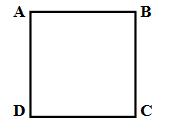
\includegraphics[width=0.3\textwidth]{2021SAC28.PNG}
    \end{center}

    \item %% Problem 21
    Consider a quadrilateral with vertices $A(-6,4), B(0,-8), C(6,4)$, and $D(0,12)$. This quadrilateral can be classified as a \blank.

    \item %% Problem 22
    Consider $\triangle ABC$ with point $D$ on $\overline{AB}$ such that $\overline{CD}\perp \overline{AB}$. If $m\angle ACB=78.28\degree$, $AD=9$ and $CD=12$, then $DB=\blank$. (nearest tenth)
    
    \item %% Problem 23
    Find the area of a triangle with vertices $(0,12), (0,0)$ and $(12,0)$.

    \item %% Problem 24
    If you cut nine circles out of a square piece of cardboard that measures 12 in by 12 in, how much cardboard is discarded? (nearest tenth)
    \begin{center}
        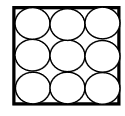
\includegraphics[width=0.3\textwidth]{2021SAC56.PNG}
    \end{center}

    \item %% Problem 25
    Russell's backyard pool is shaped like a rectangle that measures 30 ft by 50 ft. He decides to add a sidewalk that is 3 feet wide around the perimeter. Vedant, Caleb
    and Curtis will provide free labor, so he only has to pay for the concrete, which cost \$6.00 per square foot. What will the sidewalk cost?
    \begin{center}
        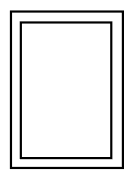
\includegraphics[width=0.3\textwidth]{2021SAC58.PNG}
    \end{center}

    \item %% Problem 26
    Find the area of the polygon below. (nearest whole number)
    \begin{center}
        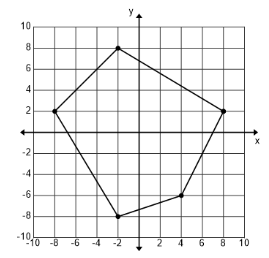
\includegraphics[width=0.3\textwidth]{2021SAC59.PNG}
    \end{center}


    The following polygon is used for problem 27 and 28.
    \begin{center}
        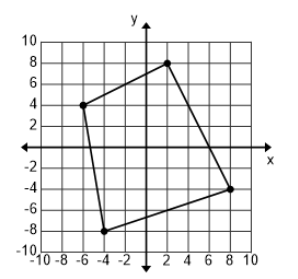
\includegraphics[width=0.3\textwidth]{2022SAC11.PNG}
    \end{center}
    \item %% Problem 27
    Find the perimeter of the polygon shown. (nearest tenth)

    \item %% Problem 28
    Find the area of the polygon shown.

    \item %% Problem 29
    Consider $\triangle ABC$ with $AB=18$ and $BC=14$. Point $D$ lies on $\overline{AC}$ such that $\overline{BD}$ bisects $\angle ABC$. 
    If $AD=10$, then $DC=\blank$. (nearest tenth)


    Use the following sketch for problems 30 and 31.
    \begin{center}
        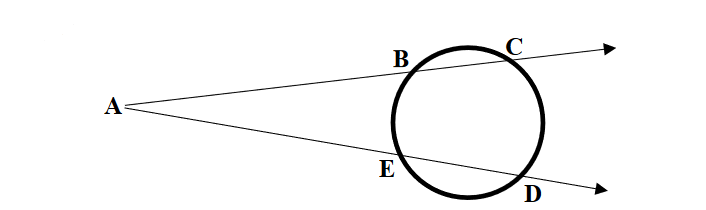
\includegraphics[width=0.3\textwidth]{2022SAC14.PNG}
    \end{center}
    \item %% Problem 30
    If $m\angle CAD=19\degree$, $mCD=120\degree$, $mDE=102\degree$, then $mBC=\blank$.

    \item %% Problem 31
    If $\overline{BD}$ intersects $\overline{CE}$ at point $P$ (not shown) with $BP=x+1$, $CP=2x$, $DP=2x+2$, and $EP=x+4$, then $CE=\blank$. (nearest tenth)

    \item %% Problem 32
    Consider a right circular cone with a base perimeter of 75 cm and a lateral area of 490 cm. Find the volume of the cone. (nearest whole number)

    \item %% Problem 33
    Consider a circle inscribed in a square with side lengths 44.6 mm. Find the area inside the square but outside the circle. (nearest whole number)

    \item %% Problem 34
    Find the perimeter of a regular decagon that can be inscribed in a circle with an area of 254 cm$^2$. (nearest tenth)


    The following diagram is used for problems 35-40.
    \begin{center}
        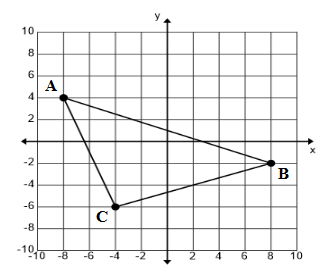
\includegraphics[width=0.3\textwidth]{2023UILSAC2.PNG}
    \end{center}
    \item %% Problem 35
    The $y$-intercept of $\overline{AB}$ is the point $P(a,b)$. $b=\blank$.

    \item %% Problem 36
    Point $D(3,d)$ lies on the perpendicular bisector of $\overline{CB}$. $d=\blank$.

    \item %% Problem 37
    The perimeter of $\triangle ABC$ is $\blank$. (nearest tenth)

    \item %% Problem 38
    The area of $\triangle ABC$ is $\blank$. (nearest tenth)

    \item %% Problem 39
    The length of the median from point $C$ to $\overline{AB}$ is $\blank$. (nearest hundredth)

    \item %% Problem 40
    $\triangle ABC$ is a/an \blank triangle.

    \item %% Problem 41
    Which of the following would best represent a two dimensional perspective of the top view of this figure shown?
    \begin{center}
        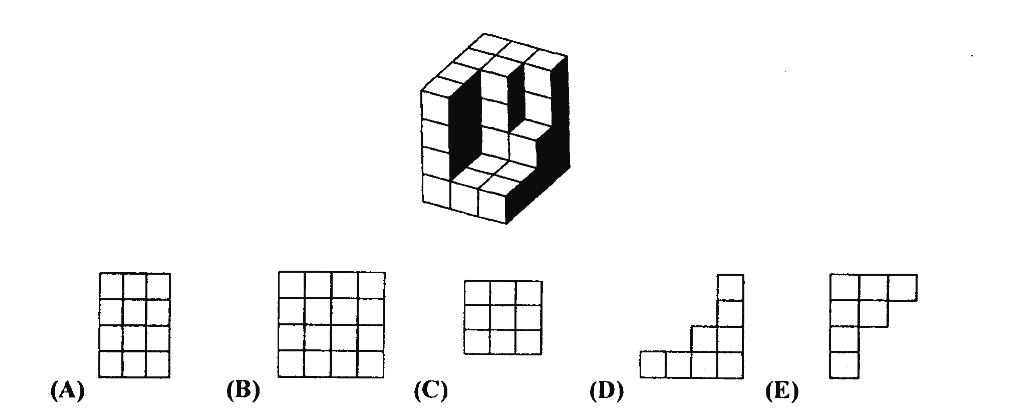
\includegraphics[width=1\textwidth]{2008SAC26.PNG}
    \end{center}

    
    For Problems 42 and 43, consider the regular polygon $ABCDEF$ with $EF=8$.
    \item %% Problem 42
    The area of the polygon is \blank. (nearest whole number)

    \item %% Problem 43
    The area of $\triangle ACE$ is \blank. (nearest whole number)

    
    Consider the following diagram for problems 44 and 45.
    \begin{center}
        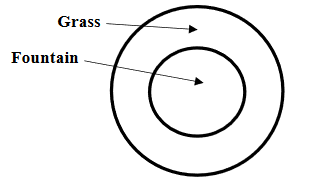
\includegraphics[width=0.3\textwidth]{2023SAC16.PNG}
    \end{center}
    Russell entertains a guest in an area of his backyard which has a magnificent fountain surrounded by an area of grass.
    The fountain area is circular with a radius of 6 feet. The grass area is the outer part of a circle with the same 
    center as the fountain and with a radius of 10 feet.
    \item %% Problem 44
    The area of the grass region is \blank square feet. (nearest whole number)

    \item %% Problem 45
    Russell decided to put up a fence along the outer perimeter of the grass region. If the fence is 
    6 feet tall and the cost of fencing is \$25/square foot, find the total cost of the fencing.

    For problems 46 and 47, consider a circle with center $O$ and diameter $\overline{BD}$. Chord $\overline{AC}$ is perpendicular to $\overline{BD}$.
    $BD=50$ and $AC=40$.
    \item %% Problem 46
    Find the area of sector $AOD$. (nearest whole number)

    \item %% Problem 47
    Find the area of the region between chord $\overline{AC}$ and minor arc $AC$. (nearest whole number)


    For problems 48 and 49 consider isosceles trapezoid $PQRS$ with $PQ=RS=10$. $\overline{QR}$ is parallel to $\overline{PS}$. 
    $QR=15$ and $PS=25$.
    \item %% Problem 48
    Find the area of $PQRS$. (nearest whole number)

    \item %% Problem 49
    $QS=\blank$. (nearest tenth)

    \item %% Problem 50
    The lateral area of a cone with a volume of 667 and a diameter of 14 is \blank. (nearest hundredth)


    For problems 51-54, consider triangle $ABC$ with vertices $A(2,8), B(6,-2)$, and $C(-4,-4)$.
    \item %% Problem 51
    Find the perimeter of triangle $ABC$. (nearest tenth)

    \item %% Problem 52
    The measure of $\angle ABC$ is \blank $\degree$. (nearest tenth)

    \item %% Problem 53
    The area of triangle $ABC$ is \blank. (nearest whole number)

    \item %% Problem 54
    Given: Triangle $ABC$ is similar to triangle $DEF$. If $EF=6.9$, then $DF=\blank$. (nearest tenth)


    For problems 55-57, you are given: Circle with center $O$, diameter $\overline{CD}$, chord $\overline{EF}$ parallel to $\overline{CD}$. $CD=20$ and $EF=16$. $m\angle COE<90\degree$.
    \item %% Problem 55
    If $H$ is the midpoint of $\overline{EF}$, then $OH=\blank$. (nearest tenth)

    \item %% Problem 56
    The area of sector $COE$ is \blank. (nearest tenth)

    \item %% Problem 57
    The arclength of minor arc $EF$ is \blank. (nearest tenth)

    \item %% Problem 58
    A right circular cylinder has a diameter of 22 and a volume of 10,264. The total surface area of the cylinder is \blank. (nearest whole number)


    For problems 59 and 60, consider isosceles trapezoid $PQRS$ with $PQ=RS=13$. $\overline{QR}$ is parallel to $\overline{PS}$. $QR=16$ and $PS=26$.
    \item %% Problem 59
    The area of trapzeoid $PQRS$ is \blank. (nearest whole number)

    \item %% Problem 60
    $PR=\blank$. (nearest tenth)

    \item %% Problem 61
    The diagonal of a television screen measures 54.12 inches. The width of the rectangularly shaped 
    television screen is 23 inches greater than the height. The area of the television screen is \blank in$^2$. (nearest whole number)

    \item %% Problem 62
    $\triangle ABC$ is similar to $\triangle FDE$. $AB=20, BC=35, DF=12$, and $DE=21$. Which of the following is a false statement?

    $\textbf{(A) } \angle B \cong \angle D \qquad \textbf{(B) } \angle C \cong \angle E \qquad \textbf{(C) } \angle A \cong \angle D \qquad \textbf{(D) } \frac{AC}{EF}=\frac{5}{3} \qquad \textbf{(E) } \frac{DE}{BC}=\frac{3}{5}$

    \item %% Problem 63
    If the height of a right cylindrical container is doubled and the diameter is cut in half, then 
    the ratio of the volume of the original container to the volume of the new container is? 

    \item %% Problem 64
    What is the perimeter of this hexagon? All lengths are in cm.
    \begin{center}
        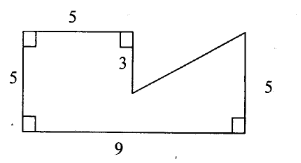
\includegraphics[width=0.5\textwidth]{2006B24.PNG}
    \end{center}

    \item %% Problem 65
    The coordinates of the vertices of $\triangle ABC$ are $C(0,7), B(2,5)$, and $A(x,2)$. 
    $\angle ABC$ is a right angle if $x$ equals:

    \item %% Problem 66
    The center of a circle inscribed in a triangle is caleld the \blank.

    \item %% Problem 67
    $\overline{NQ}$ is an altitude of $\triangle MNO$. $NM = 13$ cm, $NO = 15$ cm, and $NQ = 12$ cm. The perimeter of $\triangle MNO$ is 

    \item %% Problem 68
    If $(6,9)$ and $(10,3)$ are the coordinates of two opposite vertices of a square, which of the following is one of the other vertices of the square?

    \item %% Problem 69
    The drawing contains $\triangle ABC$, a right triangle, and three squares attached to 
    $\triangle ABC$. Find the sum of the areas of the four triangles.
    \begin{center}
        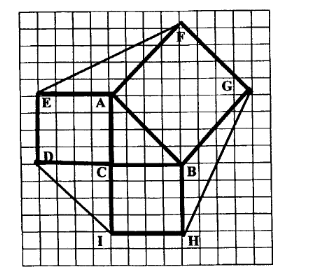
\includegraphics[width=0.3\textwidth]{2006B60.PNG}
    \end{center}

    \item %% Problem 70
    The area of a rectangle is 300 cm$^2$. The ratio of its length to its width is 4:3. The perimeter of the rectangle is: 

    \item %% Problem 71
    Find the radius of the circle. (nearest tenth)

    \begin{center}
        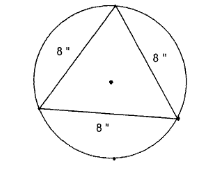
\includegraphics[width=0.3\textwidth]{2008B8.PNG}
    \end{center}

    \item %% Problem 72
    $\angle P$ is supplementary to $\angle Q$ and $\angle R$ is complementary to $\angle S$. If $m\angle P=75\degree$ and 
    $m\angle Q=3\times m\angle R$, then $m\angle S=$?

    \item %% Problem 73
    A triangle is drawn as shown. Find the height, $h$, if $YZ=18$'', $m\angle YZX = 30\degree$, and $XZ=12$''.
    \begin{center}
        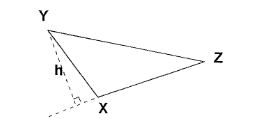
\includegraphics[width=0.4\textwidth]{2008B15.PNG}
    \end{center}

    \item %% Problem 74
    Which of the following nets when folded will not form a cube?
    \begin{center}
        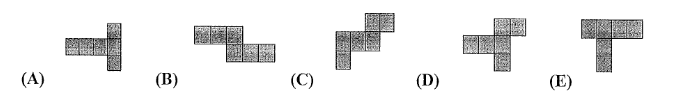
\includegraphics[width=0.6\textwidth]{2008B26.PNG}
    \end{center}

    \item %% Problem 75
    A tangent and a secant intersect at point $A$ in the exterior of a circle. The measures of the two intercepted arcs are 
    75$\degree$ and 50$\degree$. What is the measure of angle $A$ formed by the tangent and the secant?

    \item %% Problem 76
    Two legs of a triangle have lengths of 10 cm and 15 cm with an included angle of $30\degree$. Find the area of the triangle.

    \item %% Problem 77
    Rene drew this quadrilateral on the coordinate plane below. The coordinates of the vertices are integers. What is the area of his quadrilateral?
    \begin{center}
        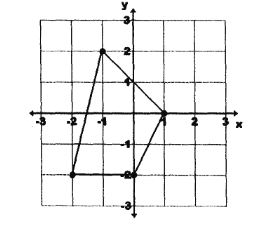
\includegraphics[width=0.3\textwidth]{2009A7.PNG}
    \end{center}

    \item %% Problem 78
    If a line in the plane of a circle is perpendicular to a radius at its endpoint on the circle then the line is \blank to the circle.

    \item %% Problem 79
    $\angle A$ and $\angle B$ are complementary. The ratio of $m\angle A$ to $m\angle B$ is 4:5. Find the ratio of $m\angle B$ to its supplement.

    \item %% Problem 80
    The length of the sides of each of the small cubes is 1 cm. How many of the small cubes would need to be added to this figure 
    to make a rectangular prism that is 4 cm long, 3 cm wide, and 2 cm tall?
    \begin{center}
        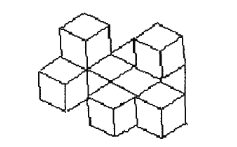
\includegraphics[width=0.3\textwidth]{2009A12.PNG}
    \end{center}

    \item %% Problem 81
    Find the lateral area, nearest square cm, of the oblique cylinder.
    \begin{center}
        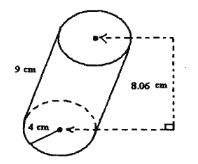
\includegraphics[width=0.3\textwidth]{2009A33.PNG}
    \end{center}

    \item %% Problem 82
    Let $AB$ be the diameter of the circle with center $C$ with $CG\perp AB$, $DE\perp AB$, and $EF\perp DF$. If $AE=9$ and $BE=4$ then $DF=$?
    \begin{center}
        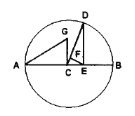
\includegraphics[width=0.3\textwidth]{2009A47.PNG}
    \end{center}

    \item %% Problem 83
    Points $A$, $B$, $C$, and $D$ are the vertices of a square. Point $E$ is on the interior of the square such that points 
    $A$, $B$, and $E$ form an equilaterial triangle. A line segment connects point $D$ and $E$. Another line segment connects points $C$ and $E$. Find $m\angle CED$.

    \item %% Problem 84
    The coordinates of the vertices of $\triangle ABC$ are $(-1,2),(1,0)$ and $(-2,-2)$. The medians of the $\triangle ABC$ intersect at $(x,y)$. Find $x+y$.

    \item %% Problem 85
    Deputy Dawg is building two adjacent rectangular pens to hold his puppies. Each pen has a length 3 times longer than its width and the pens share a common side (width).
    He has 65 feet of fencing. What will the area of each pen be?

    \item %% Problem 86
    If a quadrilateral is inscribed in a circle, then its opposite angles are \blank .

    \item %% Problem 87
    The coordinates of the vertices of $\triangle ABC$ are $(-2,0), (1,4)$, and $(4,0)$. The coordinates of the incenter is:

    \item %% Problem 88
    Shirley Knott is filling up her circular wading pool. The diameter of the pool is 6 feet and the height of the pool is 1 foot. What is the 
    maximum number of whole gallons of water can she use and not cause the pool to overflow?

    \item %% Problem 89
    The vertex angle of an obtuse isosceles triangle has a measure of 100$\degree$ and the length of one the sides adjacent 
    to the vertex angle is 4 cm. Find the area of the triangle. (nearest tenth)

    \item %% Problem 90
    Given the trapezoid shown with bases $a$ and $b$, the length of segment $PQ$ is the \blank mean of $a$ and $b$.
    \begin{center}
        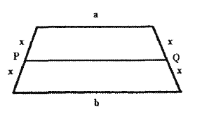
\includegraphics[width=0.4\textwidth]{2009B25.PNG}
    \end{center}

    \item %% Problem 91
    Adjacent dots on the grid are 1 cm apart when measured vertically and horizontally. Find the area of the shaded figure shown.
    \begin{center}
        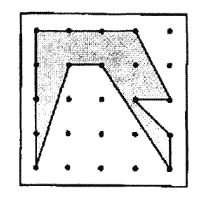
\includegraphics[width=0.3\textwidth]{2009B28.PNG}
    \end{center}

    \item %% Problem 92
    Two chords, $WY$ and $XZ$ intersect in the interior of a circle at point $P$ such that 
    $m\angle WPX=70\degree$ and $m\arc{WX}=120\degree$. If points $X$ and $Y$ are not on $\arc{WZ}$ then $m\arc{YZ}$ is:

    \item %% Problem 93
    Find the lateral area, nearest square cm, of the cone.
    \begin{center}
        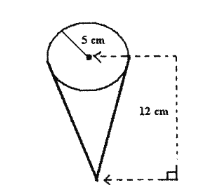
\includegraphics[width=0.3\textwidth]{2009B41.PNG}
    \end{center}

    \item %% Problem 94
    Which of the following would best represent a two dimensional perspective of the front right side view of this figure shown?
    \begin{center}
        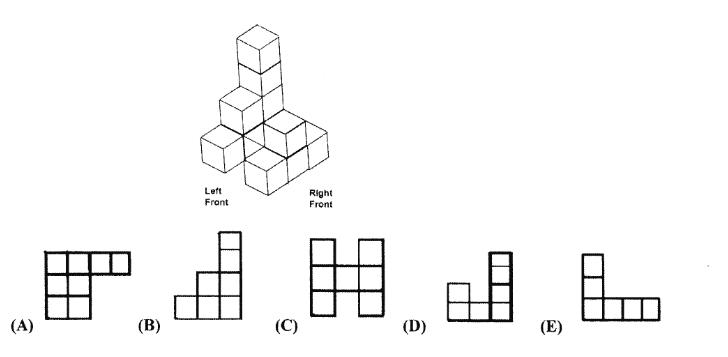
\includegraphics[width=0.7\textwidth]{2009B54.PNG}
    \end{center}

    \item %% Problem 95
    Find the lateral surface area of this prism. All angles are right angles.
    \begin{center}
        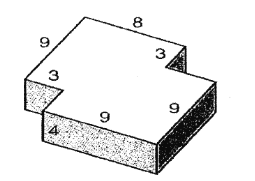
\includegraphics[width=0.4\textwidth]{2009B60.PNG}
    \end{center}

    \item %% Problem 96
    A right cylinder water tank is 6 feet high and has an inside radius of 3 feet. The amount of water 
    in the tank is 75\% of its maximum capacity. How much water is in the tank? (nearest gallon)

    \item %% Problem 97
    The region bounded by two radii of a circle and their intercepted arc is called a:

    \item %% Problem 98
    One-centimeter cubes are glued together to form the object in the figure shown. The two-dimensional persepctive of the top view 
    of this figure has a perimeter of: 
    \begin{center}
        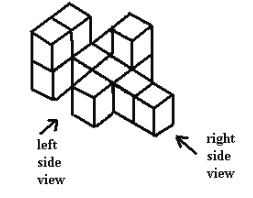
\includegraphics[width=0.3\textwidth]{2010A11.PNG}
    \end{center}

    \item %% Problem 99
    $\angle A$ and $\angle B$ are complementary angles. $\angle A$ and $\angle C$ are supplementary angles.
    Find $m\angle C$ if $m\angle A=2x-5$ and $m\angle B=x+2$.

    \item %% Problem 100
    Find $AD$ if $AB=90$ cm. and $AC=50$ cm. (nearest cm)
    \begin{center}
        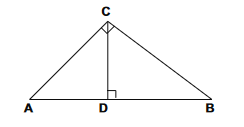
\includegraphics[width=0.3\textwidth]{2010A40.PNG}
    \end{center}

    \item %% Problem 101
    The area of a right isosceles triangle is 12.5 cm$^2$. Its perimeter is: (nearest tenth).

    \item %% Problem 102
    $\overline{AB}$, $\overline{AC}$, $\overline{BD}$, and $\overline{CD}$ are chords of circle $O$ and point $E$ lies on circle $O$. Which of the following is a true statement?
    \begin{center}
        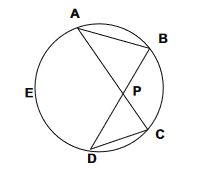
\includegraphics[width=0.3\textwidth]{2010A52.PNG}
    \end{center}

    $\textbf{(A) } m\angle ABD = \frac{1}{2}\times m\arc{AED} \qquad \textbf{(B) } m\angle BPC = \frac{1}{2}\times m\arc{CB} \qquad \textbf{(C) } m\angle ACD = 2\times m\arc{AED} \qquad \textbf{(D) }m\angle APD = m\angle ABP + m\angle DCP \qquad \textbf{(E) } m\angle ABP + m\angle BDC$

    \item %% Problem 103
    A regular polygon has $S$ sides and $D$ diagonals. If the polygon had one more side, $S+1$, it would have $D+10$ diagonals. The polygon is a:

    \item %% Problem 104
    Matt and Nick constructed two buildings using identical cubes. Matt's building weighs 200 g, and Nick's building weighs 600 g. How many of the cubes in Nick's building are hidden and cannot be seen in the figure?
    \begin{center}
        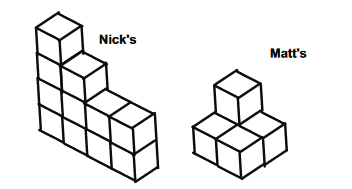
\includegraphics[width=0.3\textwidth]{2010A60.PNG}
    \end{center}

    \item %% Problem 105
    Which of the following are the side lengths of a scalene acute triangle?

    $\textbf{(A) } 9,40,41 \qquad \textbf{(B) } 4,7,11 \qquad \textbf{(C) } 9,10,11 \qquad \textbf{(D) } 5,5,8 \qquad \textbf{(E) } 8,7,14$

    \item %% Problem 106
    The point $(6,-6)$ is rotated 60 degrees clockwise about the origin. The coordinates of the point after the rotation is \blank . (closest approximation)

    \item %% Problem 107
    In $\triangle PRS, QT // RS, RS=4, QT=3, ST=x$, and $PT=x+5$. Find $PS$.
    \begin{center}
        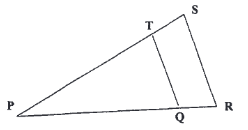
\includegraphics[width=0.3\textwidth]{2010B10.PNG}
    \end{center}

    \item %% Problem 108
    If two parallel lines are intersected by a transversal, then the alternate angles are \blank .

    \item %% Problem 109
    $\triangle ABC$ and $\triangle PQR$ exist such that $AB=BC=PQ=PR, m\angle ABC = 2x\degree, m\angle QPR = x\degree$, and they have equal areas. Find $x$.

    \item %% Problem 110
    A circle with a center at $C$ has a radius of 9 cm. A chord $AB$ of the circle is 6 cm long. Find the distance from the chord to the center $C$.

    \item %% Problem 111
    Find the perimeter of $\triangle XYZ$ if $XY=8$'', $XZ=11$'' and $m\angle XYZ=120\degree$. (nearest tenth)
    \begin{center}
        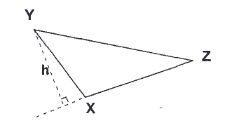
\includegraphics[width=0.3\textwidth]{2010B53.PNG}
    \end{center}

    \item %% Problem 112
    Polygon $ABCDEF$ is a regular hexagon and segments $AE$ and $CF$ intersect at point $Z$. The ratio of the area of triangle $EFZ$ to the area of the quadrilateral $ABCZ$ is:
    \begin{center}
        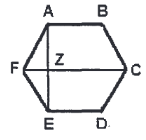
\includegraphics[width=0.3\textwidth]{2010B58.PNG}
    \end{center}

    \item %% Problem 113
    Find the perimeter of $\triangle BCD$. (nearest tenth)
    \begin{center}
        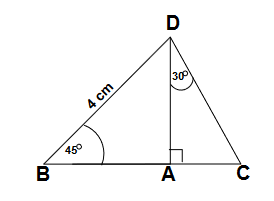
\includegraphics[width=0.3\textwidth]{2018A9.PNG}
    \end{center}

    \item %% Problem 114
    Max Space has a rectangular sheet of cardboard that is 4 feet by 6 feet. He is going to cut out a 5 inch square from each of the four corners, 
    then fold up the sides, tape edges, and make a rectangular box without a top. What is the volume of the box? (nearest tenth)

    \item %% Problem 115
    Given: $\triangle ABE$ is similar to $\triangle DON$; $\angle A \cong \angle N$; $\angle B\cong \angle D$; $AB=30$ cm; $DN=24$ cm; and $NO=16$ cm. Find $AE$.

    \item %% problem 116
    $\triangle ABC$ is a scalene triangle. Point $P$ lies on segment $AB$ such that segment $CP$ is the altitude of the triangle, $m\angle CBP=65\degree$, $AP=12$'', $BP=15$''. Find $m\angle ACP$. (nearest degree)

    \item %% 117
    Find the radius of the circle inscribed in $\triangle ABC$ with $AC=3$'', $AB=4$'', and $BC=5$''.
    \begin{center}
        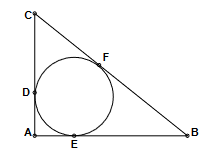
\includegraphics[width=0.3\textwidth]{2018A47.PNG}
    \end{center}

    \item %% 118
    Find the area of the rhombus shown given that $AC-BD=4$''
    \begin{center}
        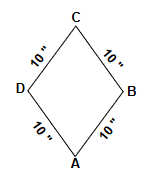
\includegraphics[width=0.3\textwidth]{2018A53.PNG}
    \end{center}

    \item %% 119
    Find the sum of $x,y$, and $z$, given the degree measures of the angles shown.
    \begin{center}
        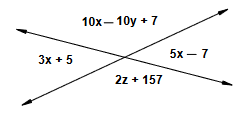
\includegraphics[width=0.3\textwidth]{2018A60.PNG}
    \end{center}

    \item %% 120
    $\overline{AB}, \overline{AC}, \overline{BD}$, and $\overline{CD}$ are chords of circle $O$ and point $E$ lies on circle $O$. Find $m\arc{AED}$ given $m\angle BPC = 95\degree$ and $m\angle BAP = 25\degree$.
    \begin{center}
        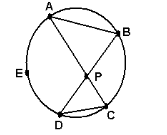
\includegraphics[width=0.3\textwidth]{2018B9.PNG}
    \end{center}

    \item % 121
    $\angle A$ and $\angle B$ are supplementary angles with $m\angle A = 5x-4$ and $m\angle B = 3x+2$. Find the 
    absolute value difference in the measures of $\angle A$ and $\angle B$.

    \item % 122
    An $8\times 27$ rectangle is split into four triangles, as shown below, by three line segments which divide the rectangle's longer sides into segments of lengths 6 and 21. How long is the dotted segment?
    \begin{center}
        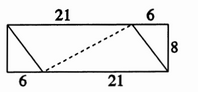
\includegraphics[width=0.3\textwidth]{txml13.PNG}
    \end{center}

    \item % 123
    A square is split into four triangles, and then three of the four triangles are shaded, as shown. If the areas of the shaded triangles are 3, 4, and 6, as shown, what is the area of the unshaded triangle?
    \begin{center}
        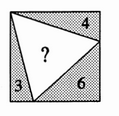
\includegraphics[width=0.3\textwidth]{txml26.PNG}
    \end{center}

    \item % 124
    Find $DC$ if $AE=3$''.
    \begin{center}
        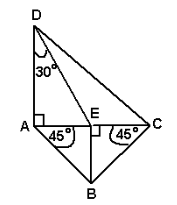
\includegraphics[width=0.3\textwidth]{2018B18.PNG}
    \end{center}

    \item % 125
    Which of the following points of concurrency are always on the exterior of an obtuse triangle
    
    (1) circumcenter \qquad (2) centroid \qquad (3) incenter \qquad (4) orthocenter

    \item % 126
    An elongated square pyramid is a nonahedron. It has 9 faces and 9 vertices. How many edges does it have?

    \item % 127
    Points $P(-1,1), Q(3,5), R(17,1)$, and $S(x,y)$ are the coordinates of the vertices of a parallelogram. How many possible coordinates of $S$ exist for the fourth vertex?

    \item % 128
    Given the regular pentagon shown, find $BC$ with $AC+AD+BE+BD+CE=44.5''$. (nearest tenth)
    \begin{center}
        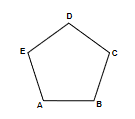
\includegraphics[width=0.3\textwidth]{2018B58.PNG}
    \end{center}

    \item % 129
    Leo Oiler drew a polyhedron with 7 faces and 11 edges. How many vertices does it have?

    \item % 130
    Two lines are \blank ? \blank if and only if the product of their slopes is -1.

    \item % 131
    Find $m\angle APB$. (drawing is not to scale)
    \begin{center}
        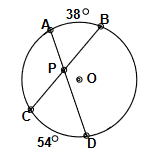
\includegraphics[width=0.3\textwidth]{2019A11.PNG}
    \end{center}

    \item % 132
    A right cylinder can of Papi Spinach has a diameter length of 4'' and a height of 5''. What is the total surface area of the spinach can? (nearest tenth)

    \item % 133
    Find the perimeter this hexagon? All lengths are in cm.
    \begin{center}
        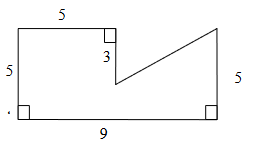
\includegraphics[width=0.3\textwidth]{2019A17.PNG}
    \end{center}

    \item % 134
    Find the area of the shaded figure.
    \begin{center}
        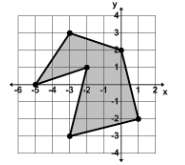
\includegraphics[width=0.3\textwidth]{2019A33.PNG}
    \end{center}

    \item % 135
    The length of the base of $\triangle PQR$ is 40 cm. and the height is 60 cm. $\triangle ICU$ is formed by cutting off 
    25\% of the base of $\triangle PQR$ and adding 20\% of the height of $\triangle PQR$. The area of $\triangle ICU$ is what percent of $\triangle PQR$?


    Consider isosceles trapzeoid $ABCD$ for problems 136 and 137. $\overline{EF}$ is the median.
    $BC=BE=12$. $m\angle BAD = 80\degree$.
    \begin{center}
        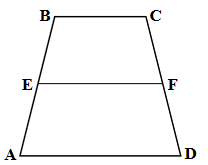
\includegraphics[width=0.3\textwidth]{2023District11.PNG}
    \end{center}

    \item % 136
    Draw auxiliary line segment $\overline{EC}$. Find the area of triangle $EBC$. (nearest tenth)

    \item % 137
    Find the area of trapezoid $ABCD$. (nearest whole number)


    Consider the circle with center $O$ and diameter $\overline{GH}$ for problems 138 and 139.
    The measure of minor arc $GJ=110\degree$ and $GH=18$.
    \begin{center}
        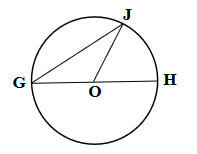
\includegraphics[width=0.3\textwidth]{2023District13.PNG}
    \end{center}

    \item % 138
    The area of sector $JOH$ is \blank. (nearest tenth)

    \item % 139
    The perimeter of triangle $GOJ$ is \blank. (nearest tenth)

    \item % 140
    A regular hexagon is inscribed in a circle. If the area of the circle is 452, then the perimeter of the hexagon is \blank. (nearest whole number)

    \item % 141
    The area of the three-quarter circle is 530. Find the perimeter of the three-quarter circle. (nearest whole number)
    \begin{center}
        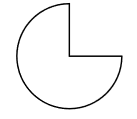
\includegraphics[width=0.3\textwidth]{2023District16.PNG}
    \end{center}

    \item % 142
    A right circular cone has a radius of 7.75 and a total surface area of 462. Find the volume of the cone. (nearest whole number)

    \item % 143
    Consider right triangle $ABC$ with $m\angle C = 90\degree$. Point $D$ lies on $\overline{AB}, \overline{CD}\perp \overline{AB}$, $AC=6$ and $AB=10$.
    Find the area of triangle $ACD$. (nearest hundredth)

    \item % 144
    Find the area of a triangle with vertices $A(6,4,2), B(8,6,10)$, and $C(6,2,8)$. (nearest tenth)    
    
    
    For problems 145-147 consider the points $A(-6,2), B(8,4), C(2,-6)$ and $D(-10,-4)$.
    \item % 145
    Find the distance from point $A$ to the midpoint of $\overline{BC}$ (nearest tenth).

    \item % 146
    Given: $\overleftrightarrow{AC}$ is parallel to $\overleftrightarrow{DE}$. If the coordinates of point $E$ are $(a,2)$, then $a=\blank$.
    
    \item % 147
    Given: $\overleftrightarrow{FG}$ is the perpendicular bisector of $\overleftrightarrow{AB}$. If the coordinates of $F$ are $(3,b)$, then $b=\blank$.

    \item % 148
    Consider the circle below. If $AB=14$, $BC=18$, and $AE=16$, then $DE=\blank$. 
    \begin{center}
        \includegraphics[width=0.3\textwidth]{2024State10.PNG}
    \end{center}

    \item % 149
    Consider equilaterial triangle $PQR$ with a circumscribed circle. If the area of the circle is 339, then the area of triangle $PQR$ is \blank. (nearest whole number)

    \item % 150
    Consider the circle below. If the measure of minor arc $HK=128\degree$ and the measure of $\angle GFJ=33\degree$, then the measure of minor arc $GJ=\blank$.
    \begin{center}
        \includegraphics[width=0.3\textwidth]{2024State12.PNG}
    \end{center}

    \item % 151
    The total area of a cylinder with a radius of 14 cm is 3343 cm$^2$. The volume of the cylinder is $\blank$ cm$^3$. (nearest whole number)

    \item % 152
    Consider the circle below with center $O$. Chord $\overline{AC}$ intersects diameter $\overline{BD}$ at point $E$. $\overline{AC}\perp \overline{BD}, BD=18$, and $AC=14$. $BE=\blank$. (nearest tenth)
    \begin{center}
        \includegraphics[width=0.3\textwidth]{2024State14.PNG}
    \end{center}

    \item % 153
    Given: $\triangle ABC$ is inscribed in a circle with $m\angle C=90\degree$, $AC=7$, and the perimeter of the triangle is 56. The area of the circle = \blank. (nearest whole number)

    \item % 154
    Consider $\triangle ABC$ with $m\angle ABC = 90\degree$. Point $D$ lies on $\overline{AC}$ such that $m\angle ABD = 90\degree$. If $AD=6$ and $CD=13$, then the perimeter of $\triangle ABC = \blank$. (nearest tenth)


    Use the following circle for problems 155 and 156. The circle shown has an area of 707. The measure of $\angle BAC=30\degree$. Point $O$ is the center of the circle.
    \begin{center}
        \includegraphics[width=0.3\textwidth]{2024State17.PNG}
    \end{center}
    \item % 155
    Find the area of $\triangle AOC$. (nearest tenth)

    \item % 156
    Find the area of the region bounded by chord $\overline{BC}$ and minor arc $BC$. (nearest tenth)


    For problems 157-159, use the given: $\triangle ABC$ is similar to $\triangle DEF$, $AB=36, BC=39,AC=42$, and $DF=28$.
    \item % 157
    Point $G$ is the midpoint of $\overline{DF}$. $EG=\blank$. (nearest tenth)

    \item % 158
    Point $H$ lines on $\overline{AC}$ and ray $\overrightarrow{BH}$ bisects $\angle ABC$. $AH=\blank$. (nearest hundredth)

    \item % 159
    The area of $\triangle BHC=\blank$. (nearest whole number)

    \item % 160
    Consider $\overleftrightarrow{AB}$ such that every point on $\overleftrightarrow{AB}$ is the same distance from point $P(-6,4)$ as the distance from point $Q(8,-2)$. If point $R(13,c)$ lies on $\overleftrightarrow{AB}$, then $c=\blank$. (nearest tenth)

    \item % 161
    If two parallel lines are cut by a transversal, then each pair of consecutive interior angles is/are:

    \item % 162
    Given the tangent and secant shown, find $x$. (nearest tenth)
    \begin{center}
        \includegraphics[width=0.3\textwidth]{2019B9.PNG}
    \end{center}

    \item % 163
    Horace Troff bought a water tank for his cattle. The tank was in the shape of a rectangular prism without the top. It was 3 feet deep, 2 feet wide, and 8 feet long. How many gallons of water would it take to fill it to the top without spilling over?

    \item % 164
    Find the perimeter of this pentagon.
    \begin{center}
        \includegraphics[width=0.3\textwidth]{2019B14.PNG}
    \end{center}

    \item % 165
    Which of the following are the side lengths of an obtuse triangle?

    $\textbf{(A) } 6,8,9 \qquad \textbf{(B) } 5,6,7 \qquad \textbf{(C) }4,4,4\sqrt{2}\qquad \textbf{(D) } 3,3\sqrt{3},6\qquad \textbf{(E) } 8,8,12$

    \item % 166
    Which of the following points of concurrency is on a side of a right triangle but not a vertex point, on the interior of an acute triangle, and on the exterior of an obtuse triangle? 

    \item % 167
    Find $DC$ if $CE=5''$.
    \begin{center}
        \includegraphics[width=0.3\textwidth]{2019B29.PNG}
    \end{center}

    \item % 168
    Points $P$ and $R$ are on a circle with center $C$ such that $m\angle PCR=94\degree$. Point $Q$ lies outside of the circle such that $QP$ and $QR$ are tangent to the circle. Find $m\angle PQR$.

    \item % 169
    Find the volume of the figure shown. (nearest tenth)
    \begin{center}
        \includegraphics[width=0.3\textwidth]{2019B34.PNG}
    \end{center}

    \item % 170
    Which of these trapezoidal means are used for finding the volume of a frustum of a cone?

    \item % 171
    The triangle shown is considered to be which of the following types of triangles?
    \begin{center}
        \includegraphics[width=0.3\textwidth]{2021A5.PNG}
    \end{center}

    \item % 172
    Find the area of $\triangle ABC$. (nearest tenth)
    \begin{center}
        \includegraphics[width=0.3\textwidth]{2021A7.PNG}
    \end{center}

    \item % 173
    If the square of the length of the longest side of a triangle is less than the sum of the squares of the lengths of the other two sides, then the triangle is a(n) \blank triangle.

    \item % 174
    Sir Cal Puhl is pouring a rectangular concrete patio to put his circular hot tub on. The diameter of the hot tub is 10 feet. The dimensions of the patio is 14 feet by 18 feet. What percent of the area of the patio is covered by the tub? (nearest whole percent)

\end{enumerate}

\section*{Solutions}
\begin{enumerate}[label=\bfseries\arabic*.]
    \item %% Problem 1
    Right 

    \item %% Problem 2
    44 cm$^2$

    \item %% Problem 3
    7.5 units$^2$

    \item %% Problem 4
    8 units$^2$

    \item %% Problem 5
    95 cm$^2$

    \item %% Problem 6
    $(-3,-3)$

    \item %% Problem 7
    70$\degree$

    \item %% Problem 8
    6 cm$^2$

    \item %% Problem 9
    15.3 cm 

    \item %% Problem 10
    50 units 

    \item %% Problem 11
    $n^2-1$

    \item %% Problem 12
    6

    \item %% Problem 13
    9.4

    \item %% Problem 14
    5.0

    \item %% Problem 15
    342

    \item %% Problem 16
    7.75 

    \item %% Problem 17
    29$\degree$

    \item %% Problem 18
    523

    \item %% Problem 19
    143

    \item %% Problem 20
    648

    \item %% Problem 21
    kite 

    \item %% Problem 22
    10.6

    \item %% Problem 23
    72

    \item %% Problem 24
    30.9 in$^2$

    \item %% Problem 25
    \$3096.00

    \item %% Problem 26
    148

    \item %% Problem 27
    47.2

    \item %% Problem 28
    136

    \item %% Problem 29
    7.8

    \item %% Problem 30
    56$\degree$

    \item %% Problem 31
    5.5

    \item %% Problem 32
    793 cm$^3$

    \item %% Problem 33
    427 mm$^2$

    \item %% Problem 34
    55.6 cm
    
    \item %% Problem 35
    1

    \item %% Problem 36
    -7

    \item %% Problem 37
    40.5

    \item %% Problem 38
    68.0

    \item %% Problem 39
    8.06

    \item %% Problem 40
    obtuse 

    \item %% Problem 41
    A 

    \item %% Problem 42
    166

    \item %% Problem 43
    83

    \item %% Problem 44
    201

    \item %% Problem 45
    \$9,424.78

    \item %% Problem 46
    692

    \item %% Problem 47
    280

    \item %% Problem 48
    173

    \item %% Problem 49
    21.8

    \item %% Problem 50
    324.67

    \item %% Problem 51
    34.4

    \item %% Problem 52
    79.5 

    \item %% Problem 53
    54

    \item %% Problem 54
    9.1

    \item %% Problem 55
    6.0

    \item %% Problem 56
    32.2

    \item %% Problem 57
    18.5

    \item %% Problem 58
    2626

    \item %% Problem 59
    252

    \item %% Problem 60
    24.2

    \item %% Problem 61
    1200

    \item %% Problem 62
    C 

    \item %% Problem 63
    2:1 

    \item %% Problem 64
    32 cm

    \item %% Problem 65
    -1

    \item %% Problem 66
    Incenter 

    \item %% Problem 67
    42 cm 

    \item %% Problem 68
    $(5,4)$

    \item %% Problem 69
    32 sq. units 

    \item %% Problem 70
    70 cm 

    \item %% Problem 71
    4.6''

    \item %% Problem 72
    55$\degree$

    \item %% Problem 73
    9''

    \item %% Problem 74
    E 

    \item %% Problem 75
    $12.5\degree$

    \item %% Problem 76
    37.5 cm$^2$

    \item %% Problem 77
    7 units$^2$

    \item %% Problem 78
    tangent 

    \item %% Problem 79
    2:7

    \item %% Problem 80
    14

    \item %% Problem 81
    226 cm$^2$

    \item %% Problem 82
    $5\frac{7}{13}$

    \item %% Problem 83
    $\frac{5\pi}{6}$

    \item %% Problem 84
    $-\frac{2}{3}$

    \item %% Problem 85
    $56\frac{1}{3}$ sq. ft. 

    \item %% Problem 86
    supplementary

    \item %% Problem 87
    $(1,1\frac{1}{2})$

    \item %% Problem 88
    211

    \item %% Problem 89
    7.9 cm$^2$

    \item %% Problem 90
    arithmetic

    \item %% Problem 91
    7 cm$^2$

    \item %% Problem 92
    $20\degree$

    \item %% Problem 93
    204 cm$^2$

    \item %% Problem 94
    B 

    \item %% Problem 95
    192 units$^2$

    \item %% Problem 96
    952 gal 

    \item %% Problem 97
    sector 

    \item %% Problem 98
    18 cm

    \item %% Problem 99
    $123\degree$

    \item %% Problem 100
    28 cm 

    \item %% Problem 101
    17.1 cm 

    \item %% Problem 102
    A 

    \item %% Problem 103
    undecagon 

    \item %% Problem 104
    4

    \item %% Problem 105
    B 

    \item %% Problem 106
    $(5.1,-8.2)$

    \item %% Problem 107
    10

    \item %% Problem 108
    supplementary

    \item %% Problem 109
    30

    \item %% Problem 110
    $6\sqrt{2}$ cm 

    \item %% Problem 111
    22.7''

    \item %% Problem 112
    1:3

    \item %% Problem 113
    11.7 cm 

    \item %% Problem 114
    6.8 cu. ft. 

    \item %% Problem 115
    20 cm

    \item %% Problem 116
    $20\degree$

    \item %% 117
    1''

    \item % 118
    96 in$^2$

    \item %% 119
    -3

    \item %120
    $140\degree$

    \item % 121
    $39.5\degree$

    \item % 122
    17

    \item % 123
    11

    \item % 124
    $3\sqrt{7}$ in 

    \item % 125
    1 \& 4 

    \item % 126
    16

    \item % 127
    3

    \item %128
    5.5''

    \item % 129
    6

    \item % 130
    perpendicular
    
    \item % 131
    $46\degree$

    \item % 132
    88.0 in$^2$

    \item % 133
    32 cm 

    \item % 134
    18 units$^2$

    \item % 135
    90\%

    \item % 136
    70.9

    \item % 137
    382

    \item % 138
    49.5

    \item % 139
    32.7

    \item % 140
    72

    \item % 141
    101

    \item % 142
    511

    \item % 143
    8.64

    \item % 144
    15.4

    \item % 145
    11.4

    \item % 146
    -16

    \item % 147
    -11

    \item % 148
    12

    \item % 149
    140

    \item % 150
    $62\degree$

    \item % 151
    14,780

    \item % 152
    3.3

    \item % 153
    491

    \item % 154
    45.4

    \item % 155
    97.4

    \item % 156
    20.4

    \item % 157
    20.7

    \item % 158
    20.16

    \item % 159
    338

    \item % 160
    29.0

    \item % 161
    supplementary 

    \item % 162
    5.0''

    \item % 163
    359 gal 

    \item % 164
    32''

    \item % 165
    E

    \item % 166
    circumcenter 

    \item % 167
    $5\sqrt{7}$ in 

    \item % 168
    $86\degree$

    \item % 169
    $193.7$ in$^3$

    \item % 170
    Heronian 

    \item % 171
    Right and Isosceles 

    \item % 172
    $27.0$ in$^2$

    \item % 173
    acute 

    \item % 174
    31\% 

\end{enumerate}



\end{document}